
\section{Testing on Synthetic Social Networks}

In this section, I test my gradient descent and Newton-CG solutions on synthetic graphs that are not produced
via a range-dependent system.
In particular, I generate these graphs using a trend commonly noticed in social media networks.
If two people in a network are friends, then their friends are also likely to become friends.
This idea is known to create 3-cliques or triangles throughout the graph.
More generally, this tends to create even larger cliques throughout the graph, as mostly-adjacent 3-cliques will
combine to create larger cliques over time.

Applying this idea, I synthetically created an initial graph with 5\% of all edges present.
Then, I apply the following for 100 evolutions:
\begin{itemize}
    \item $\alpha (u, v) = 0.02 + k*0.06$. $k$ is the number of common neighbors between $u$ and $v$
    \item $\omega (u, v) = 0.03$
\end{itemize}

Using these rates, random friendships are more likely to disappear than reappear.
However, friendships that are created via a common friend are far more likely than anything.
This leads to clique-esque structures in the graph.

\begin{figure}
    \begin{minipage}{0.49\textwidth}
        \begin{center}
            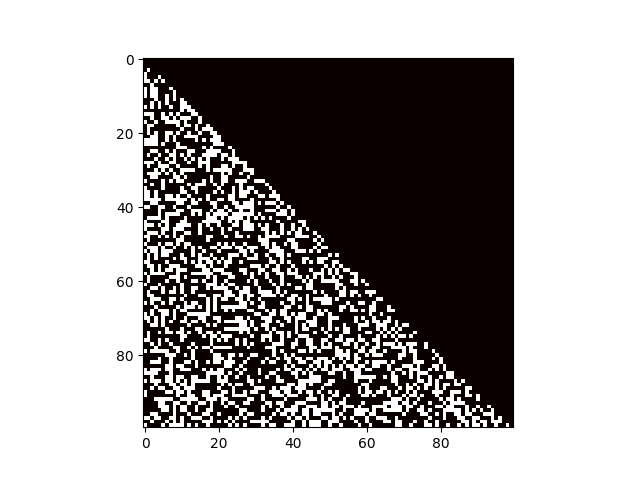
\includegraphics[scale=0.5]{figures/original-linear.png}
        \end{center}
    \end{minipage}
    \begin{minipage}{0.49\textwidth}
        \begin{center}
            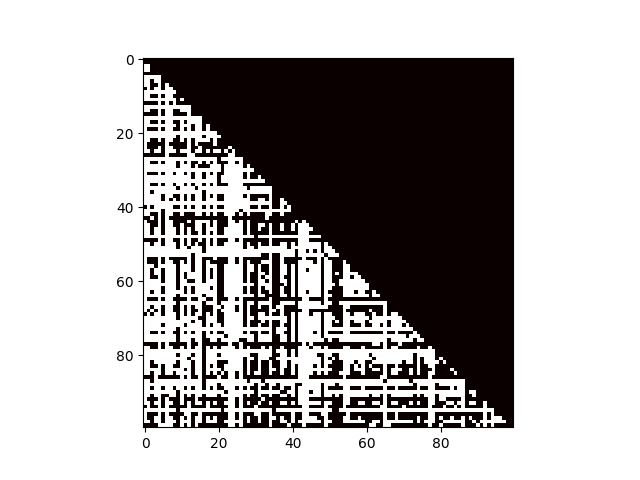
\includegraphics[scale=0.5]{figures/scg-linear.png}
        \end{center}
    \end{minipage}
	\caption{
        Left: State 100 of the original social graph.
        Right: State 100 of the graph predicted using gradient descent.
	}
    \label{fig:sgd-social-linear}
\end{figure}

\begin{figure}
    \begin{minipage}{0.49\textwidth}
        \begin{center}
            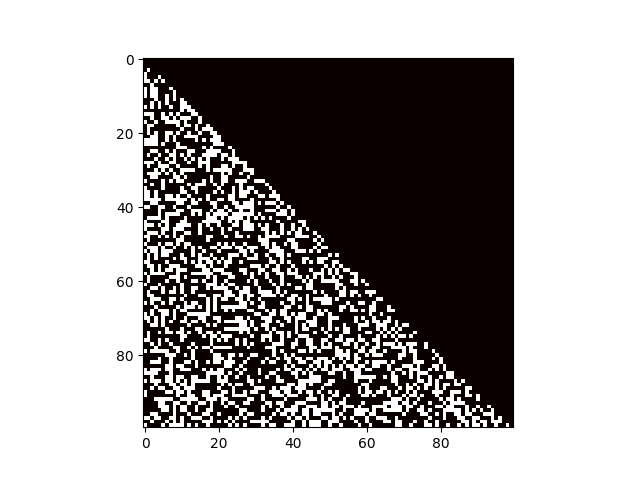
\includegraphics[scale=0.5]{figures/original-linear.png}
        \end{center}
    \end{minipage}
    \begin{minipage}{0.49\textwidth}
        \begin{center}
            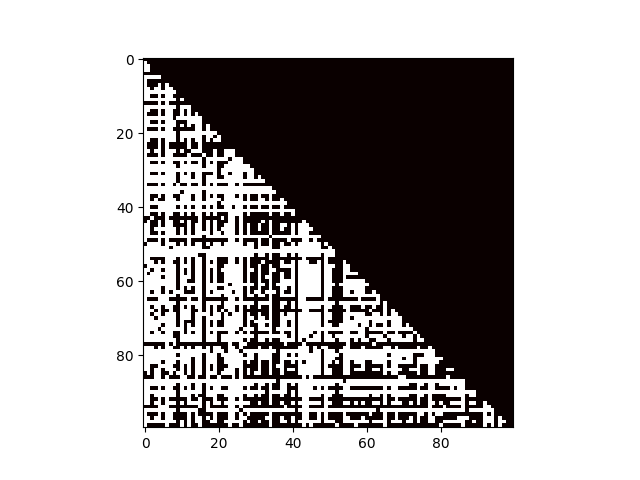
\includegraphics[scale=0.5]{figures/newton-linear.png}
        \end{center}
    \end{minipage}
	\caption{
        Left: State 100 of the original social graph.
        Right: State 100 of the graph predicted using the Newton Conjugate Gradient algorithm.
	}
    \label{fig:newton-social-linear}
\end{figure}

Following this generation of evolutions, I run the first 50 evolutions through my gradient descent and Newton-CG algorithms.
Then, I produce a prediction of the next 50 evolutions using the models created by the algorithms.
Figure~\ref{fig:sgd-social-linear} and Figure~\ref{fig:newton-social-linear} show the results for these experiments using a birth function of $0.2 * 0.8^k$, where $k$ is the range between two vertices.
These results generated a graph which was far too connected, which I was quite surprised about.

\begin{figure}
    \begin{minipage}{0.49\textwidth}
        \begin{center}
            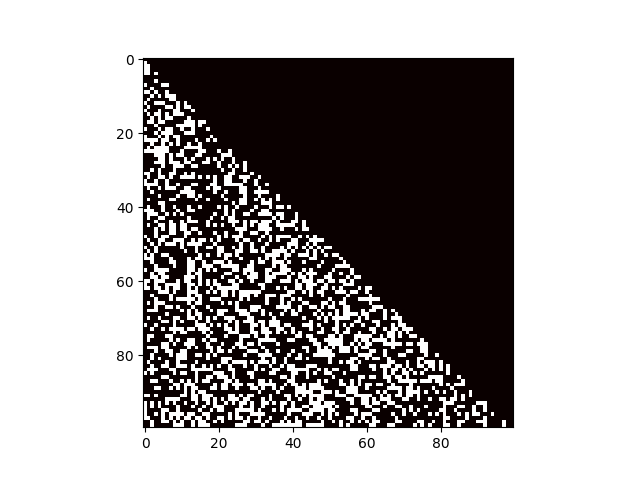
\includegraphics[scale=0.5]{figures/original-square.png}
        \end{center}
    \end{minipage}
    \begin{minipage}{0.49\textwidth}
        \begin{center}
            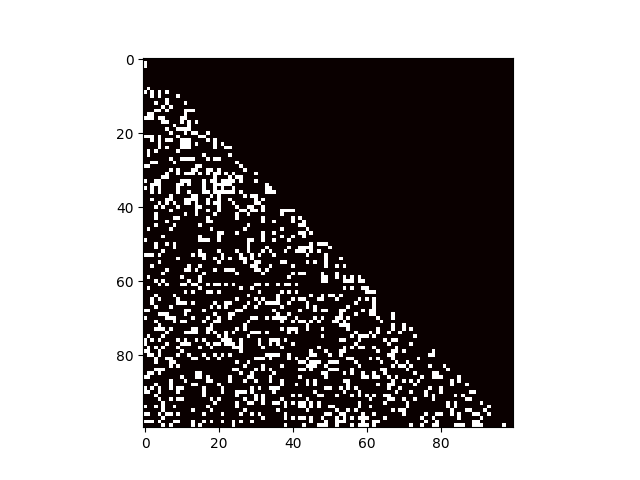
\includegraphics[scale=0.5]{figures/scg-square.png}
        \end{center}
    \end{minipage}
	\caption{
        Left: State 100 of the original social graph.
        Right: State 100 of the graph predicted using gradient descent and a quadratic birth rate.
	}
    \label{fig:sgd-social-square}
\end{figure}

\begin{figure}
    \begin{minipage}{0.49\textwidth}
        \begin{center}
            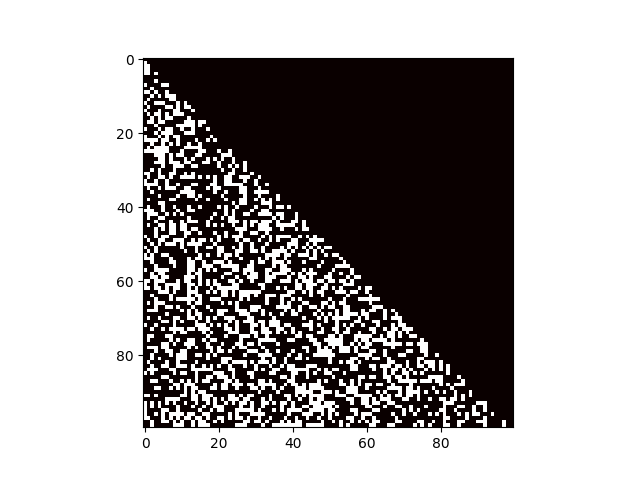
\includegraphics[scale=0.5]{figures/original-square.png}
        \end{center}
    \end{minipage}
    \begin{minipage}{0.49\textwidth}
        \begin{center}
            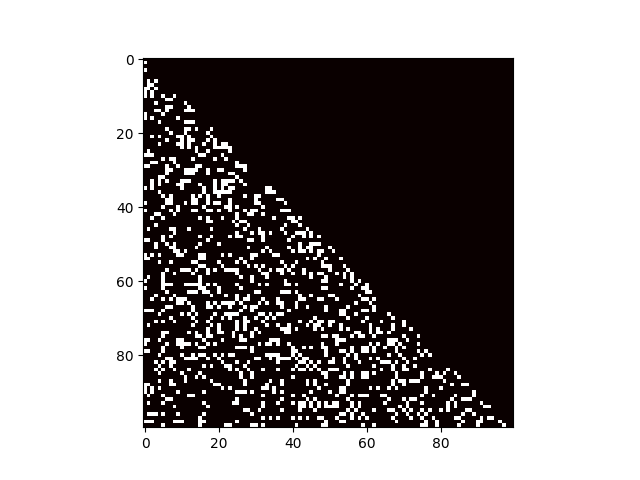
\includegraphics[scale=0.5]{figures/newton-square.png}
        \end{center}
    \end{minipage}
	\caption{
        Left: State 100 of the original social graph.
        Right: State 100 of the graph predicted using the Newton Conjugate Gradient algorithm and a quadratic birth rate.
	}
    \label{fig:newton-social-square}
\end{figure}


Figure~\ref{fig:sgd-social-square} and Figure~\ref{fig:newton-social-square} shows the results for these experiments using a birth function of $0.2 * 0.97^(k^2)$.
These results seem to match far better to the original.
It makes sense that using a sense of range to indicate likelier friendships works in this scenario to an extent,
but I am surprised that it worked so well.
The results are still a bit sparser than the original graph, but overall these seem surprisingly accurate.
I would be interested to see if this holds on larger datasets if the algorithms would work on those instances.

\section{Conclusion}

Overall, I am reasonably pleased with these results.
I feel that the algorithms I presented to solve the inverse problem at hand are reasonable.
My gradient descent algorithm is very accurate but takes a long time to run.
My Newton-CG algorithm is not as accurate but runs surprisingly fast, such that even the model itself is slower to compute.
Following these restrictions, I think that these approaches seem to solve the inverse problem I chose to tackle quite well.

Given more time, there are a few more points that I would like to explore:
\begin{itemize}
    \item Applying the DBAR method to this problem. I think it's possible that this algorithm could run as fast as Newton-CG
          and get more accurate results, but this is untested. A similar inverse problem solved in a case study from class
          uses this algorithm to great effect.
    \item Applying my algorithms to more scientific data (for example, a protein-protein network). Finding data to do this
          on was difficult given the problem size restriction, but if I could find something in the area I would be very interested
          to test on it
    \item I'd like to do more research on approaches to evolving graphs. I'm unsure that these other approaches involve inverse problems,
          so I did not find them appropriate to try in this project, but I would find them interesting to investigate nonetheless.
\end{itemize}